\documentclass[12pt,a4paper]{article}
\usepackage{graphicx}
\usepackage{hyperref}
\title{1-s2.0-S2352146518302606-main self driving — Research Booklet}
\date{}
\begin{document}
\maketitle
\tableofcontents
\newpage
\section{1. Introduction}
Here's a simple summary:

Autonomous vehicles (AVs) are becoming a reality and will have a big impact on many areas of life. Researchers are studying how AVs will affect things like traffic, jobs, and the environment. One of the biggest concerns is how AVs will make decisions in dangerous situations, as they will be programmed to follow ethical guidelines rather than human instincts. This paper looks at the current state of AV technology and its potential effects on traffic, the environment, and society. It also discusses the challenges that need to be overcome, such as ensuring user privacy and preventing hacking.

Further reading: https://scholar.google.com/scholar?q=1.+Introduction
\begin{figure}[h]
\centering
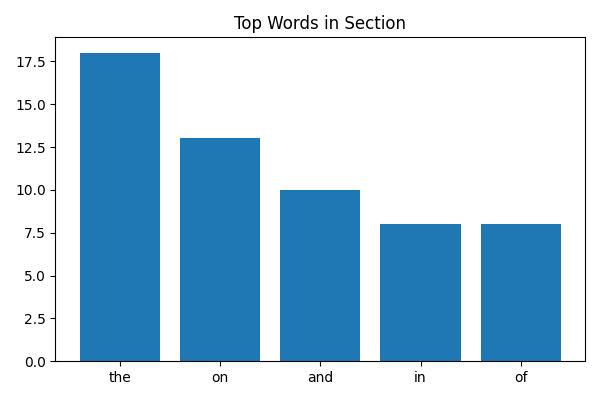
\includegraphics[width=0.8\textwidth]{D:\projects\mp 2 rag\autonomous rag\outputs\visual_605dd2c1c7f540b7b811849d03351659.png}
\end{figure}
\section{2. AVs technological perspective}
Here's a summary of the section in clear and simple terms:

**Autonomous Vehicles**

There are 6 levels of autonomous vehicles, from 0 (traditional) to 5 (fully autonomous). Level 3 is a key milestone, where the vehicle takes over monitoring the environment and can drive itself to some extent. Level 5 is the ultimate goal, where the vehicle can drive itself in all conditions, without human intervention.

**How Autonomous Vehicles Work**

Autonomous vehicles have 4 main parts:

1. **Sensing system**: Collects data from the environment using various sensors, like LIDAR (which creates 3D maps) and GPS.
2. **Client system**: Processes the data in real-time to make decisions, using powerful computers and software.
3. **Action system**: The mechanical parts of the vehicle, like steering and braking, which will be improved for autonomous driving.
4. **Human-machine interface**: Provides information to the driver, and will be minimalist in fully autonomous vehicles.

**Cooperative Autonomous Driving**

Autonomous vehicles need to communicate with each other, the infrastructure, the cloud, and other devices to work efficiently and safely. This is known as V2X communication. A robust and reliable communication network is needed to transmit data quickly and securely.

**Infrastructure Improvements**

Road infrastructure will need to be improved to support autonomous vehicles, with clear road signs, smooth road layouts, and V2I technologies that allow vehicles to communicate with the infrastructure.

**Challenges and Future**

While some autonomous vehicles are already available, fully autonomous vehicles (Level 5) are still a long way off. Many technical challenges need to be overcome, including developing reliable communication networks and improving infrastructure.

Further reading: https://arxiv.org/search/?query=2.+AVs+technological+perspective&searchtype=all
\begin{figure}[h]
\centering
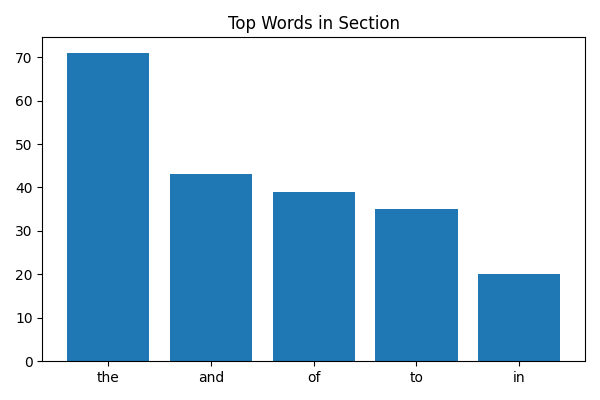
\includegraphics[width=0.8\textwidth]{D:\projects\mp 2 rag\autonomous rag\outputs\visual_51dd4728c4d445b29c8a16ed64c744df.png}
\end{figure}
\section{3. Effects of AVs on mobility}
Here's a summary of the section in clear and simple terms:

**Traffic Efficiency**

* The first self-driving cars were programmed to drive very cautiously, which could lead to increased congestion on roads.
* To solve this, self-driving cars need to be able to communicate with each other and make cooperative decisions to improve traffic flow.
* One way to do this is through "platooning," where self-driving cars travel together in a group at high speeds with small gaps between them.
* This would require advanced traffic management strategies, which are still being developed and tested.

**Mobility Rate and Patterns**

* More people are using car-sharing and ride-hailing services, which could lead to a decrease in the number of privately owned vehicles on the road.
* Self-driving cars could support these services and make them more efficient, which could lead to a decrease in the overall number of vehicles on the road.
* However, some researchers think that self-driving cars could also lead to an increase in the number of miles driven, as people may use them more frequently.

**Safety-Related Aspects**

* Self-driving cars have the potential to greatly reduce the number of accidents on the road, since most accidents are caused by human error.
* However, there are still risks associated with self-driving cars, such as the possibility of hacking or cyber attacks.
* Governments are working to develop secure systems to prevent these types of attacks.
* Self-driving cars could also lead to new safety risks, such as passengers becoming overconfident and not wearing seatbelts.

Further reading: https://scholar.google.com/scholar?q=3.+Effects+of+AVs+on+mobility
\begin{figure}[h]
\centering
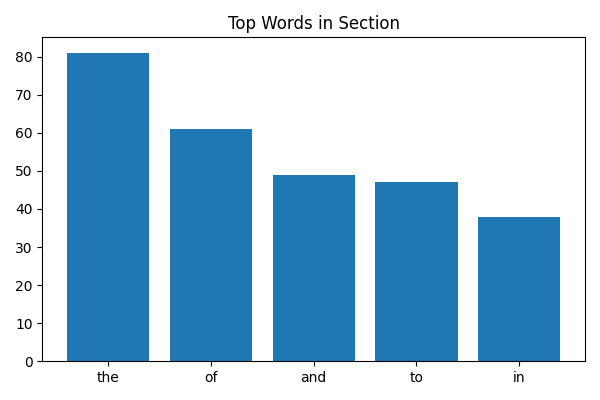
\includegraphics[width=0.8\textwidth]{D:\projects\mp 2 rag\autonomous rag\outputs\visual_41b512d9b37745459833e103c236bff1.png}
\end{figure}
\section{4. Further considerations about AVs}
Here's a summary of the section in clear and simple terms:

The widespread adoption of self-driving cars (AVs) will depend on many factors beyond just transportation. Some of these factors include:

* Environmental concerns: AVs will likely increase the use of electric vehicles, which will help reduce pollution and energy consumption.
* Urban planning: AVs may lead to urban sprawl, so city planners need to ensure that green spaces are protected and cities are designed sustainably.
* Public acceptance: Some people may be hesitant to use AVs due to concerns about safety, data privacy, and job loss. Educational campaigns can help address these concerns.
* Policy and legislation: Governments need to create new laws and regulations to govern the use of AVs, including issues like liability in accidents and data privacy.
* Job market impact: AVs may replace some jobs, but they will also create new opportunities in fields like technology and communications.
* Data management: The collection and sharing of data from AVs needs to be regulated to ensure security, privacy, and transparency.

Overall, the transition to AVs will require a coordinated effort from governments, industries, and individuals to address these various challenges and ensure a smooth and beneficial transition.

Further reading: https://www.semanticscholar.org/search?q=4.%20Further%20considerations%20about%20AVs
\begin{figure}[h]
\centering
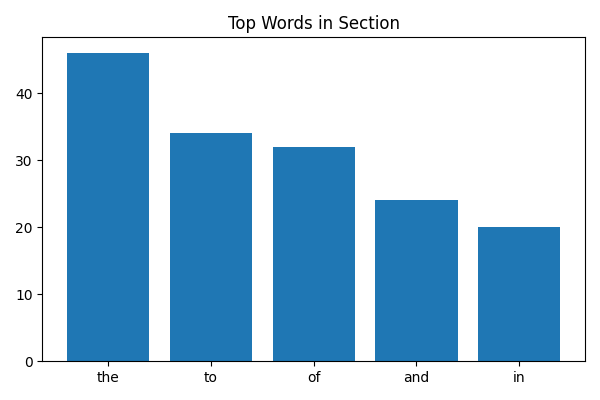
\includegraphics[width=0.8\textwidth]{D:\projects\mp 2 rag\autonomous rag\outputs\visual_e5365bde458d4bf695eeb3507a8d1472.png}
\end{figure}
\section{5. Conclusions}
Here's a summary of the section in clear and simple terms:

Self-driving cars (AVs) could make transportation better in many ways, such as making it more efficient, safe, clean, and accessible to everyone. However, for this to happen, certain conditions need to be met. If not, self-driving cars might not bring the benefits we want. Since fully self-driving cars won't be available for sale soon, we need to use this time to plan how traffic will work with these cars and make sure we're ready for the changes they'll bring. We also need to think about the legal and ethical issues surrounding self-driving cars, so we can make sure society is ready for them.

Further reading: https://arxiv.org/search/?query=5.+Conclusions&searchtype=all
\begin{figure}[h]
\centering
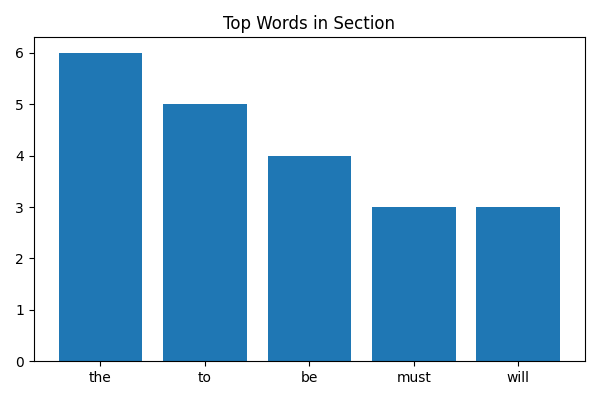
\includegraphics[width=0.8\textwidth]{D:\projects\mp 2 rag\autonomous rag\outputs\visual_78b81c1a4b3d43758ae7092fa9076f4d.png}
\end{figure}
\section{6. Acknowledgements}
Here is a summary of the section in clear, simple terms:

This research was partly paid for by the Spanish government's Ministry of Economy, Industry and Competitiveness. The authors also want to thank Marcel Sala for his helpful comments that made the paper better.

Further reading: https://arxiv.org/search/?query=6.+Acknowledgements&searchtype=all
\begin{figure}[h]
\centering
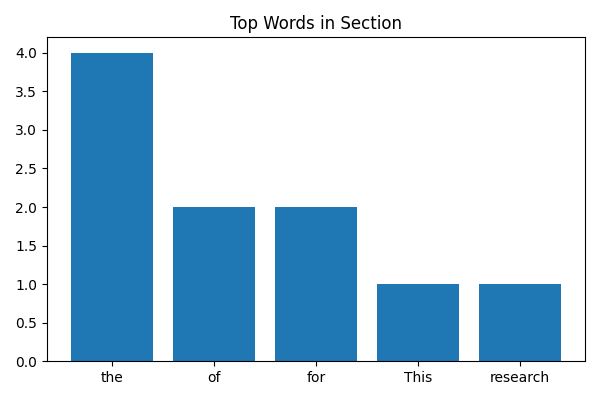
\includegraphics[width=0.8\textwidth]{D:\projects\mp 2 rag\autonomous rag\outputs\visual_08df875781a3466a90dd31504cd7913b.png}
\end{figure}
\section{7. References}
This is a list of references related to autonomous vehicles, vehicular clouds, and connected driving. The references include research papers, reports, and articles from various sources, including academic journals, government agencies, and private companies.

The topics covered in these references include:

* The architecture and applications of vehicular cloud networks
* The challenges and opportunities of autonomous vehicles, including their impact on urban mobility, traffic management, and the automotive industry
* The role of connected vehicles in improving traffic flow and reducing emissions
* The development of cooperative traffic management strategies and the assessment of their benefits
* The safety and security issues related to autonomous vehicles
* The potential impacts of autonomous vehicles on transportation planning and policy
* The development of standards and definitions for autonomous driving systems
* The analysis of strategies for truck platooning and the effects of low-speed limits on freeway traffic flow
* The future of mobility and the role of autonomous vehicles in shaping it

Overall, these references provide a comprehensive overview of the current state of research and development in the field of autonomous vehicles and connected driving.

Further reading: https://www.semanticscholar.org/search?q=7.%20References
\begin{figure}[h]
\centering
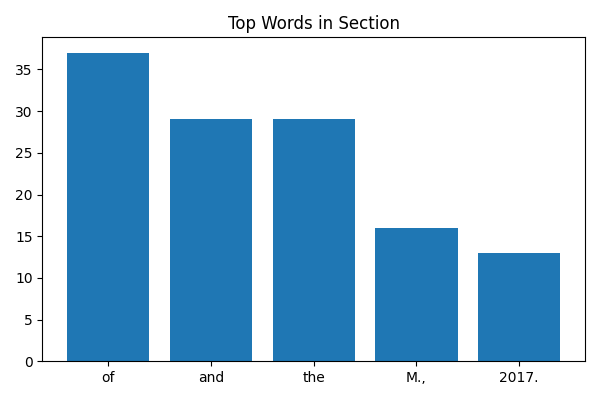
\includegraphics[width=0.8\textwidth]{D:\projects\mp 2 rag\autonomous rag\outputs\visual_0a45513ab25248bf988f3b8053e896ad.png}
\end{figure}
\end{document}